%%%%%%%%%%%%%%%%%%%%%%%%%%%%%%%%%%%%%%%%%%%%%%%%%%%%%%%%%%%
% Organización del proyecto
\section{Organización del proyecto}\label{organizacion:organizacion-del-proyecto}

Dado que el proyecto será manejado por distintas personas en distintos sistemas operativos, es vital mantener una coherencia en la estructura y el orden de los archivos y directorios del proyecto.

A continuación se presenta una propuesta base que considera tanto los ficheros del código como los del diseño artístico:

\subsection{Árbol de directorios}\label{organizacion:arbol-de-directorios}

\begin{itemize}
\item \textbf{Design:} Esta carpeta contiene todos los archivos relacionados al desarrollo artístico de los distintos componentes audiovisuales del juego tales como música, sonidos, sprites, tilesets, bocetos, dibujos, animación, etc. Es de uso interno para artistas y desarrolladores, y debe mantenerse organizada bajo reestructuración regular en el tiempo. \emph{Ningún archivo dentro de esta carpeta debe ser referenciado por el código}, por lo mismo permite mayor libertad en los nombres de los archivos. Más información al respecto en el apartado \nameref{organizacion:nombres-de-archivos}.

\item \textbf{docs:} Contiene toda la documentación de librerías, licencias, \lsc{API}, \lsc{SDK}, apuntes, notas de compilación y configuración relevante para el desarrollo del software.

\item \textbf{export:} Contiene binarios para distintas plataformas del juego y librerías necesarias para su compilación (Por ejemplo librerías propietarias para generar binarios de una consola).

\item \textbf{locales:} Todos los ficheros relativos a la i18n, es decir la carpeta que utilizarán los traductores y desde donde el juego debe tomar los strings y assets correspondientes.

\item \textbf{src:} Probablemente la carpeta principal para el desarrollo técnico. Además del código fuente del programa, contendrá todo lo relativo a nodos, escenas y scripts de Godot.

Debido a que ésta será la misma estructura que se usará
dentro de Godot, es preferible que la carpeta de la escena, además de contener el archivo \lsc{TSCN}, contenga todo lo necesario dentro de sí misma para evitar problemas de dependencia.

Si se detecta que muchas escenas están utilizando los mismos sprites, probablemente se trate de archivos que deberían procesarse e ir dentro de la carpeta shared (detallada a continuación).

\begin{itemize}
	\item \textbf{characters:} Contiene las subcarpetas \lsc{FSM}, enemies, npc y player.

	\item \textbf{game:} Todo lo relativo a los Managers y el funcionamiento del juego.

	\item \textbf{items:} Todo lo relativo a ítems. A priori dividir en armors, utility y weapons.

	\item \textbf{levels:} Escenas de niveles organizadas en distintas subcarpetas. Contemplar una ubicación para diversos templates.

	\item \textbf{ui:} Todo lo relativo a la escenas de interfaz gráfica.
\end{itemize}

\item \textbf{shared:} Colección de todos los assets y resources compartidos por más de una escena. Por ejemplo fuentes tipográficas, música, tilesets, sprites, assets genéricos, etc.
\end{itemize}

\subsubsection*{Diagrama del árbol.}
\begin{figure}[H]
\centering
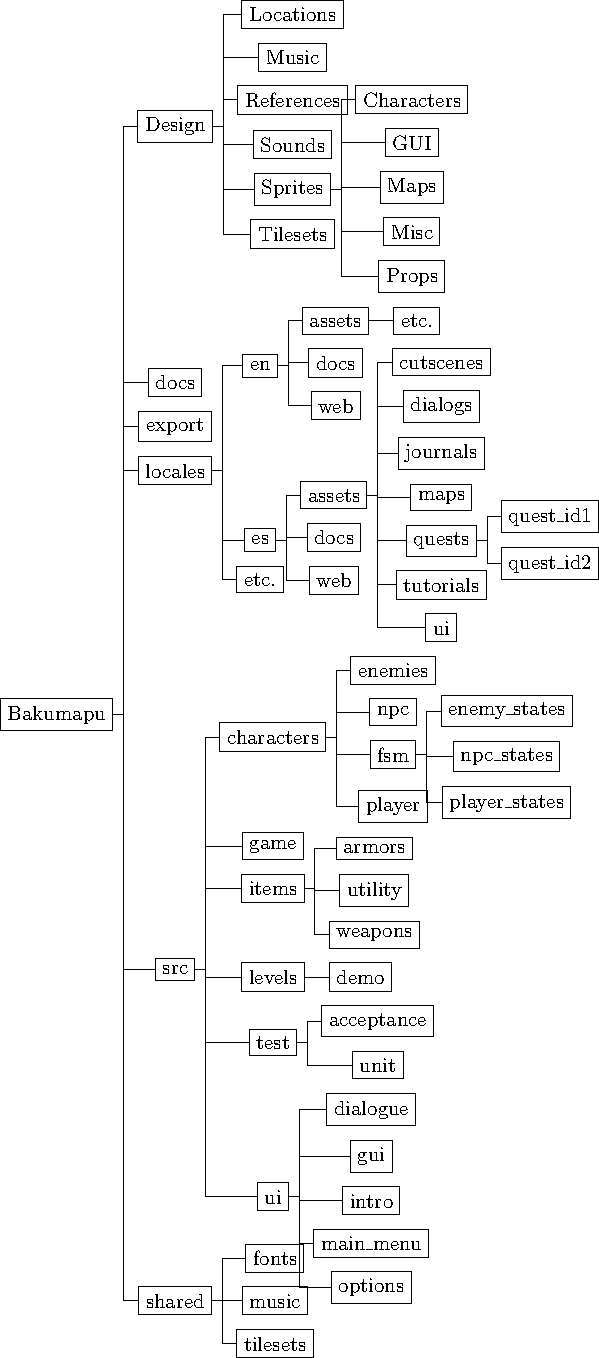
\includegraphics[height=0.93\textheight]{imágenes/arbol_proyecto}
\label{fig:arbolproyecto}
\end{figure}









\subsection{Nombres de archivos}\label{organizacion:nombres-de-archivos}
\todoii{ToDo: Criterios de nombres}{Establecer criterios de nombres de archivos}

Los nombres de archivos deben seguir ciertas especificaciones.

En la carpeta Design los nombres de los archivos pueden contener signos como eñes, acentos y mayúsculas.

\subsection{Nombres de ramas y tarjetas}\label{organizacion:nombres-de-ramas}
Ya que las ramas del repositorio \lsc{GIT} y las tarjetas del tablero Kanban tienen su origen en la misma tarea designada por el equipo de desarrollo, para mantener un seguimiento más riguroso y tener mejor información compartirán un mismo nombre. Este nombre será designado al momento de establecer la tarea y deberá cumplir las especificaciones detalladas a continuación.

% Hacer tabla resumen con códigos de nombres.
\todoii{ToDo: Tabla resumen de archivos}{Hacer tabla resumen con códigos de nombres}

Los siguientes nombres corresponden a cada subrama:
\begin{enumerate}
\item Rama de features: \lsc{ft-}
\item Rama de bugs: \lsc{bug-}
\item Rama de patches: \lsc{patch-}
Los patches son cambios al código motivados por features nuevas más que por problemas.
\end{enumerate}

Así, tareas relacionadas con algún elemento de la interfaz gráfica del juego tendrán el nombre de “ui-”

Las ramas con nombres con los que se va a interactuar son las de features y bugs.
Las ramas de nombre fijo
Hay tres tipos de subramas, ramas de features, ramas de bugs y ramas de patch
